\documentclass[11pt,a4paper]{article}

%% ── Encoding & fonts ──────────────────────────────────────────────────────────
\usepackage[T1]{fontenc}
\usepackage[utf8]{inputenc}
\usepackage{lmodern}
\usepackage{microtype}

%% ── Page geometry ─────────────────────────────────────────────────────────────
\usepackage[
  top=22mm, bottom=24mm,
  left=22mm, right=22mm,
  headheight=14pt
]{geometry}

%% ── Colour ────────────────────────────────────────────────────────────────────
\usepackage[table]{xcolor}
\definecolor{SurgBlue}{HTML}{1B3A5C}
\definecolor{SurgTeal}{HTML}{2A7F7F}
\definecolor{SurgGold}{HTML}{C08B3A}
\definecolor{SurgLight}{HTML}{EEF4F7}
\definecolor{SurgRule}{HTML}{A8C4D4}
\colorlet{SURGRULE}{SurgRule}\colorlet{SURGBLUE}{SurgBlue}\colorlet{SURGTEAL}{SurgTeal}\colorlet{SURGGOLD}{SurgGold}
\definecolor{RowAlt}{HTML}{F4F9FB}
\definecolor{HeadBg}{HTML}{1B3A5C}
\definecolor{GrayText}{HTML}{555F6D}

%% ── Graphics & drawing ────────────────────────────────────────────────────────
\usepackage{tikz}
\usetikzlibrary{positioning, calc, backgrounds}
\usepackage{graphicx}

%% ── Boxes ─────────────────────────────────────────────────────────────────────
\usepackage[most]{tcolorbox}
\tcbuselibrary{skins, breakable}

%% ── Tables ────────────────────────────────────────────────────────────────────
\usepackage{booktabs}
\usepackage{tabularx}
\usepackage{array}
\usepackage{multirow}
\usepackage{colortbl}

%% ── Typography & layout ───────────────────────────────────────────────────────
\usepackage{parskip}
\usepackage{setspace}
\usepackage{enumitem}
\usepackage{titlesec}
\usepackage{fancyhdr}
\usepackage{lastpage}
\usepackage{fontawesome5}
\usepackage{hyperref}
\usepackage{amsmath}
\usepackage{amssymb}

%% ── Hyperref setup ────────────────────────────────────────────────────────────
\hypersetup{
  colorlinks=true,
  linkcolor=SurgBlue,
  urlcolor=SurgTeal,
  pdfauthor={Meridian Academic Medical Centre},
  pdftitle={Surgical Case Series Report},
  pdfsubject={Laparoscopic Sleeve Gastrectomy Outcomes},
}

%% ── Section heading styles ────────────────────────────────────────────────────
\titleformat{\section}
  {\color{SurgBlue}\large\bfseries\MakeUppercase}
  {}
  {0pt}
  {}
  [\vspace{1pt}\color{SurgRule}\hrule height 0.8pt\vspace{4pt}]

\titleformat{\subsection}
  {\color{SurgTeal}\normalsize\bfseries}
  {}
  {0pt}
  {}

\titlespacing{\section}{0pt}{14pt}{6pt}
\titlespacing{\subsection}{0pt}{10pt}{4pt}

%% ── Header / footer ───────────────────────────────────────────────────────────
\pagestyle{fancy}
\fancyhf{}
\renewcommand{\headrulewidth}{0pt}

\fancyhead[L]{%
  
\begin{tikzpicture}[remember picture, overlay]
    \fill[SurgBlue] (0,0) rectangle (\paperwidth, 10pt);
  \end{tikzpicture}%
}

\fancyhead[C]{%
  \vspace{4pt}
  \textcolor{GrayText}{\scriptsize\itshape
    Meridian Academic Medical Centre\enspace\textbullet\enspace
    Surgical Case Series\enspace\textbullet\enspace
    Laparoscopic Sleeve Gastrectomy}%
}

\fancyfoot[C]{%
  \color{GrayText}\footnotesize
  Page \thepage\ of \pageref{LastPage}
  \quad\raisebox{0.5pt}{\textcolor{SurgRule}{$\vert$}}\quad
  Confidential -- For Peer Review Only%
}

%% ── tcolorbox styles ──────────────────────────────────────────────────────────
\tcbset{
  casebox/.style={
    enhanced, breakable,
    colback=SurgLight,
    colframe=SurgBlue,
    colbacktitle=SurgBlue,
    coltitle=white,
    fonttitle=\bfseries\small,
    arc=3pt,
    boxrule=0.6pt,
    left=8pt, right=8pt, top=6pt, bottom=6pt,
    toptitle=4pt, bottomtitle=4pt,
    attach boxed title to top left={yshift=-2pt, xshift=8pt},
    boxed title style={
      colframe=SurgBlue, colback=SurgBlue,
      arc=2pt, boxrule=0pt,
      left=4pt, right=4pt, top=2pt, bottom=2pt,
    },
    drop shadow={SurgBlue!20!black!15},
  },
  tealbox/.style={
    enhanced,
    colback=SurgTeal!7,
    colframe=SurgTeal,
    arc=3pt, boxrule=0.6pt,
    left=8pt, right=8pt, top=6pt, bottom=6pt,
  },
  goldbox/.style={
    enhanced,
    colback=SurgGold!9,
    colframe=SurgGold,
    arc=3pt, boxrule=0.6pt,
    left=8pt, right=8pt, top=6pt, bottom=6pt,
    fonttitle=\bfseries\small\color{SurgGold!70!black},
    title={},
  },
  statbox/.style={
    enhanced,
    colback=SurgBlue,
    colframe=SurgBlue,
    arc=4pt, boxrule=0pt,
    left=6pt, right=6pt, top=8pt, bottom=8pt,
    halign=center,
  },
}

%% ── Misc helpers ──────────────────────────────────────────────────────────────
\newcolumntype{L}[1]{>{\raggedright\arraybackslash}p{#1}}
\newcolumntype{C}[1]{>{\centering\arraybackslash}p{#1}}
\newcolumntype{R}[1]{>{\raggedleft\arraybackslash}p{#1}}

\newcommand{\badge}[2]{%
  \tikz[baseline=(t.base)]{
    \node[fill=#1, text=white, rounded corners=2pt,
          inner sep=2pt 3pt, font=\scriptsize\bfseries] (t) {#2};
  }%
}

\newcommand{\outcome}[1]{%
  \textcolor{SurgTeal}{\faCheckCircle}\enspace\textbf{#1}%
}

\setlength{\parindent}{0pt}
\setlength{\parskip}{5pt}

%%=============================================================================
\begin{document}
%%=============================================================================

%% ─────────────────────────────────────────────────────────────────────────────
%% TITLE BLOCK
%% ─────────────────────────────────────────────────────────────────────────────
\thispagestyle{fancy}

\begin{tikzpicture}[remember picture, overlay]
  \fill[SurgBlue]
    (current page.north west)
    rectangle
    ([yshift=-52mm]current page.north east);
  \fill[SurgTeal]
    ([yshift=-52mm]current page.north west)
    rectangle
    ([yshift=-55mm]current page.north east);
  \fill[SurgGold]
    ([yshift=-55mm]current page.north west)
    rectangle
    ([yshift=-57mm]current page.north east);
\end{tikzpicture}

\vspace*{8mm}

{\color{white}
  \begin{center}
    {\fontsize{7.5pt}{10pt}\selectfont\MakeUppercase{%
      \textls[200]{Meridian Academic Medical Centre\quad\textbullet\quad
      Department of General \& Bariatric Surgery}}}\\[4pt]
    {\fontsize{20pt}{26pt}\selectfont\bfseries
      Laparoscopic Sleeve Gastrectomy}\\[3pt]
    {\fontsize{14pt}{18pt}\selectfont\color{SurgGold!85!white}
      Surgical Case Series Report}\\[6pt]
    {\fontsize{8pt}{11pt}\selectfont\color{white!80!SurgBlue}
      Retrospective Analysis\enspace\textbullet\enspace
      January 2023 -- December 2024\enspace\textbullet\enspace
      \textit{n}\,=\,18 Patients}
  \end{center}
}

\vspace{20mm}

%% ─────────────────────────────────────────────────────────────────────────────
%% REPORT METADATA ROW
%% ─────────────────────────────────────────────────────────────────────────────
\begin{minipage}[t]{0.32\textwidth}
  \begin{tcolorbox}[tealbox, title={}]
    \textcolor{GrayText}{\scriptsize\MakeUppercase{Principal Surgeon}}\\[2pt]
    {\small\bfseries\color{SurgBlue} Dr.\ Amelia Voss, FRCS}\\[1pt]
    {\scriptsize\color{GrayText} Consultant Bariatric Surgeon}\\[5pt]
    \textcolor{GrayText}{\scriptsize\MakeUppercase{Co-Investigator}}\\[2pt]
    {\small\bfseries\color{SurgBlue} Dr.\ Carlos Mendez, MD}\\[1pt]
    {\scriptsize\color{GrayText} Surgical Registrar}
  \end{tcolorbox}
\end{minipage}%
\hfill%
\begin{minipage}[t]{0.32\textwidth}
  \begin{tcolorbox}[tealbox, title={}]
    \textcolor{GrayText}{\scriptsize\MakeUppercase{Institution}}\\[2pt]
    {\small\bfseries\color{SurgBlue} Meridian Academic Medical Centre}\\[1pt]
    {\scriptsize\color{GrayText} 14 Harrow Lane, Westfield, WF2 9KT}\\[5pt]
    \textcolor{GrayText}{\scriptsize\MakeUppercase{Ethics Reference}}\\[2pt]
    {\small\bfseries\color{SurgBlue} MAMC-SURG-2023-0041}\\[1pt]
    {\scriptsize\color{GrayText} Approved by IRB Committee}
  \end{tcolorbox}
\end{minipage}%
\hfill%
\begin{minipage}[t]{0.30\textwidth}
  \begin{tcolorbox}[tealbox, title={}]
    \textcolor{GrayText}{\scriptsize\MakeUppercase{Submission Date}}\\[2pt]
    {\small\bfseries\color{SurgBlue} 15 February 2025}\\[5pt]
    \textcolor{GrayText}{\scriptsize\MakeUppercase{Report Version}}\\[2pt]
    {\small\bfseries\color{SurgBlue} v2.1\enspace--\enspace Final}\\[5pt]
    \textcolor{GrayText}{\scriptsize\MakeUppercase{Funding}}\\[2pt]
    {\scriptsize\color{GrayText} No external funding received}
  \end{tcolorbox}
\end{minipage}

\vspace{10pt}

%% ─────────────────────────────────────────────────────────────────────────────
%% ABSTRACT
%% ─────────────────────────────────────────────────────────────────────────────
\begin{tcolorbox}[
  enhanced,
  colback=SurgBlue!4,
  colframe=SurgBlue,
  arc=3pt, boxrule=0.5pt,
  left=12pt, right=12pt, top=8pt, bottom=8pt,
]
\textbf{\color{SurgBlue}Abstract.}\enspace
This retrospective case series evaluates the surgical outcomes and short-term complications
of laparoscopic sleeve gastrectomy (LSG) performed at Meridian Academic Medical Centre
between January 2023 and December 2024. Eighteen consecutive patients (mean age
$41.6 \pm 9.2$ years; mean preoperative BMI $46.3 \pm 7.1$~kg/m\textsuperscript{2})
underwent standard five-port LSG under general anaesthesia. The primary endpoint was
percentage excess weight loss (\%EWL) at 12 months. Secondary endpoints included
30-day morbidity, operative time, length of hospital stay, and resolution of obesity-related
comorbidities. Mean \%EWL at 12 months was $68.4 \pm 12.7\%$. No intraoperative deaths
occurred. Major complications (Clavien--Dindo grade\,$\geq$\,III) were observed in
$2/18$ patients ($11.1\%$). These findings support LSG as a safe and effective bariatric
procedure in a high-volume academic centre.

\smallskip
\textbf{\color{SurgTeal}Keywords:}
\textit{sleeve gastrectomy; bariatric surgery; obesity; weight loss; morbidity; case series}
\end{tcolorbox}

\vspace{6pt}

%% ─────────────────────────────────────────────────────────────────────────────
%% SECTION 1 – INTRODUCTION
%% ─────────────────────────────────────────────────────────────────────────────
\section{Introduction}

Obesity remains a global health challenge, affecting approximately 650 million adults
worldwide and increasing the risk of type\,2 diabetes, hypertension, obstructive sleep
apnoea, and cardiovascular disease. Metabolic and bariatric surgery is the most effective
long-term treatment for severe obesity, achieving sustained weight loss and significant
comorbidity resolution.

Laparoscopic sleeve gastrectomy has emerged as the most commonly performed bariatric
procedure globally, accounting for roughly $60\%$ of all primary bariatric operations.
Its relative technical simplicity, favourable risk profile, and consistent efficacy make
it particularly suitable for high-volume centres seeking standardised patient outcomes.
This report presents a retrospective case series of 18 consecutive LSG procedures
conducted at Meridian Academic Medical Centre, with the aim of documenting operative
parameters, perioperative outcomes, and 12-month weight-loss data to contribute to the
growing evidence base.

%% ─────────────────────────────────────────────────────────────────────────────
%% SECTION 2 – PATIENTS & METHODS
%% ─────────────────────────────────────────────────────────────────────────────
\section{Patients \& Methods}

\subsection{Patient Selection}

Patients were eligible if they met NICE bariatric guidelines (BMI\,$\geq 40$~kg/m\textsuperscript{2},
or $\geq 35$ with a significant comorbidity), had completed a 12-week supervised weight
management programme, and were deemed fit for general anaesthesia by a multidisciplinary
team including a bariatric surgeon, dietitian, clinical psychologist, and specialist nurse.
Exclusion criteria included prior bariatric surgery, active malignancy, untreated psychiatric
illness, or non-compliance with preoperative dietary instructions.

\subsection{Surgical Technique}

All procedures were performed by a single consultant surgeon (A.V.) using a standardised
five-trocar laparoscopic technique. The greater curvature was mobilised from the pylorus
(3~cm proximal) to the angle of His. Gastric transection was performed over a 36~Fr
bougie using a linear endoscopic stapler (Synapse MedTech SureCut Pro, 60~mm green
cartridges), reinforced with absorbable suture. A leak test was conducted intraoperatively
via methylene blue dye. Nasogastric tube and urinary catheter were removed before
recovery-room discharge.

\subsection{Outcome Measures}

\begin{itemize}[leftmargin=18pt, itemsep=2pt]
  \item \textbf{Primary:} \%EWL at 12 months post-operatively
  \item \textbf{Secondary:} Operative time (skin-to-skin), length of hospital stay (LOS),
    30-day readmission rate, complications graded by Clavien--Dindo classification,
    and resolution of comorbidities (T2DM, hypertension, OSA) at 12 months
\end{itemize}

\subsection{Statistical Analysis}

Continuous variables are expressed as mean\,$\pm$\,SD or median \lbrack IQR\rbrack{} as
appropriate. Categorical variables are presented as counts and percentages. All analyses
were performed using standard statistical methods. A $p$-value of $<0.05$ was considered
statistically significant.

%% ─────────────────────────────────────────────────────────────────────────────
%% SECTION 3 – PATIENT DEMOGRAPHICS TABLE
%% ─────────────────────────────────────────────────────────────────────────────
\section{Patient Demographics \& Baseline Characteristics}

\begin{center}
\small
\setlength{\tabcolsep}{7pt}
\renewcommand{\arraystretch}{1.35}
\begin{tabularx}{\textwidth}{L{5.4cm} C{3.2cm} C{3.2cm} C{3.2cm}}
  \rowcolor{HeadBg}
  \color{white}\bfseries Characteristic &
  \color{white}\bfseries All Patients ($n$=18) &
  \color{white}\bfseries Female ($n$=13) &
  \color{white}\bfseries Male ($n$=5) \\
  \midrule
  \rowcolor{RowAlt}
  Age, years (mean $\pm$ SD) & $41.6 \pm 9.2$ & $40.1 \pm 8.7$ & $45.8 \pm 10.3$ \\
  BMI, kg/m\textsuperscript{2} (mean $\pm$ SD) & $46.3 \pm 7.1$ & $45.7 \pm 6.8$ & $48.2 \pm 8.0$ \\
  \rowcolor{RowAlt}
  Excess weight, kg (mean $\pm$ SD) & $54.8 \pm 16.3$ & $51.2 \pm 14.9$ & $64.4 \pm 18.7$ \\
  Ideal body weight, kg (mean) & $68.0$ & $63.0$ & $83.0$ \\
  \rowcolor{RowAlt}
  ASA grade I / II / III, \% & 0 / 56 / 44 & 0 / 62 / 38 & 0 / 40 / 60 \\
  \midrule
  \rowcolor{HeadBg!20}
  \multicolumn{4}{l}{\color{SurgBlue}\small\bfseries Comorbidities at baseline}\\
  \rowcolor{RowAlt}
  Type 2 diabetes mellitus & 9 (50.0\%) & 6 (46.2\%) & 3 (60.0\%) \\
  Hypertension & 11 (61.1\%) & 8 (61.5\%) & 3 (60.0\%) \\
  \rowcolor{RowAlt}
  Obstructive sleep apnoea & 7 (38.9\%) & 4 (30.8\%) & 3 (60.0\%) \\
  GORD / reflux & 5 (27.8\%) & 4 (30.8\%) & 1 (20.0\%) \\
  \rowcolor{RowAlt}
  Dyslipidaemia & 8 (44.4\%) & 6 (46.2\%) & 2 (40.0\%) \\
  \midrule
  \rowcolor{HeadBg!20}
  \multicolumn{4}{l}{\color{SurgBlue}\small\bfseries Preoperative preparation}\\
  \rowcolor{RowAlt}
  12-wk diet programme completed & 18 (100\%) & 13 (100\%) & 5 (100\%) \\
  Liver shrinkage diet (2 wk) & 18 (100\%) & 13 (100\%) & 5 (100\%) \\
  \rowcolor{RowAlt}
  Preop weight loss, kg (mean) & $7.4$ & $6.9$ & $8.8$ \\
  \bottomrule
\end{tabularx}
\end{center}

\vspace{4pt}

%% ─────────────────────────────────────────────────────────────────────────────
%% SECTION 4 – OPERATIVE OUTCOMES
%% ─────────────────────────────────────────────────────────────────────────────
\section{Operative \& Perioperative Outcomes}

\subsection{Key Metrics Summary}

\vspace{4pt}
\begin{minipage}[t]{0.23\textwidth}
  \begin{tcolorbox}[statbox]
    {\color{SurgGold}\large\bfseries 72.4 min}\\[2pt]
    {\color{white!80!SurgBlue}\scriptsize Mean Operative Time}
  \end{tcolorbox}
\end{minipage}%
\hfill%
\begin{minipage}[t]{0.23\textwidth}
  \begin{tcolorbox}[statbox]
    {\color{SurgGold}\large\bfseries 2.1 days}\\[2pt]
    {\color{white!80!SurgBlue}\scriptsize Mean Hospital Stay}
  \end{tcolorbox}
\end{minipage}%
\hfill%
\begin{minipage}[t]{0.23\textwidth}
  \begin{tcolorbox}[statbox]
    {\color{SurgGold}\large\bfseries 11.1\%}\\[2pt]
    {\color{white!80!SurgBlue}\scriptsize Major Complication Rate}
  \end{tcolorbox}
\end{minipage}%
\hfill%
\begin{minipage}[t]{0.23\textwidth}
  \begin{tcolorbox}[statbox]
    {\color{SurgGold}\large\bfseries 68.4\%}\\[2pt]
    {\color{white!80!SurgBlue}\scriptsize Mean \%EWL at 12 mo}
  \end{tcolorbox}
\end{minipage}

\vspace{10pt}

\begin{center}
\small
\setlength{\tabcolsep}{7pt}
\renewcommand{\arraystretch}{1.35}
\begin{tabularx}{\textwidth}{L{6.0cm} C{4.5cm} C{4.5cm}}
  \rowcolor{HeadBg}
  \color{white}\bfseries Parameter &
  \color{white}\bfseries Value &
  \color{white}\bfseries Range / IQR \\
  \midrule
  \rowcolor{RowAlt}
  Operative time, min (mean $\pm$ SD) & $72.4 \pm 18.6$ & 44 -- 118 \\
  Conversion to open, $n$ (\%) & 0 (0\%) & -- \\
  \rowcolor{RowAlt}
  Intraoperative blood loss, mL & $48.3 \pm 22.1$ & 20 -- 110 \\
  Bougie size, Fr & 36 & -- \\
  \rowcolor{RowAlt}
  Staple-line reinforcement used & 18 (100\%) & -- \\
  Intraoperative leak test positive & 0 (0\%) & -- \\
  \rowcolor{RowAlt}
  Hospital LOS, days (median \lbrack IQR\rbrack) & 2.0 \lbrack 2.0--3.0\rbrack & 1 -- 5 \\
  30-day readmission & 2 (11.1\%) & -- \\
  \rowcolor{RowAlt}
  30-day mortality & 0 (0\%) & -- \\
  \bottomrule
\end{tabularx}
\end{center}

\vspace{6pt}

%% ─────────────────────────────────────────────────────────────────────────────
%% SECTION 5 – COMPLICATIONS
%% ─────────────────────────────────────────────────────────────────────────────
\section{Complications}

\begin{tcolorbox}[
  goldbox,
  title={\faExclamationTriangle\enspace Complications Graded by Clavien--Dindo Classification},
  fonttitle=\bfseries\small\color{SurgGold!80!black},
]
\small
\setlength{\tabcolsep}{6pt}
\renewcommand{\arraystretch}{1.3}
\begin{tabularx}{\linewidth}{C{1.2cm} L{4.5cm} L{5.0cm} C{1.6cm} C{1.8cm}}
  \rowcolor{SurgGold!18}
  \bfseries Grade & \bfseries Description & \bfseries Management & \bfseries $n$ & \bfseries \% \\
  \midrule
  I & Nausea / vomiting $>$48\,h & IV antiemetics, oral step-down & 3 & 16.7 \\
  \rowcolor{RowAlt}
  I & Wound seroma (port site) & Conservative, compression & 1 & 5.6 \\
  II & Urinary tract infection & Oral antibiotics & 1 & 5.6 \\
  \rowcolor{RowAlt}
  IIIa & Staple-line haemorrhage & Endoscopic haemostasis & 1 & 5.6 \\
  IIIb & Gastric leak (distal) & Re-laparoscopy, drainage & 1 & 5.6 \\
  \rowcolor{RowAlt}
  IV & -- & -- & 0 & 0 \\
  V (mortality) & -- & -- & 0 & 0 \\
  \midrule
  \rowcolor{SurgGold!10}
  \multicolumn{3}{l}{\bfseries Total any-grade complication} & 7 & 38.9 \\
  \multicolumn{3}{l}{\bfseries Major complication (grade $\geq$ III)} & 2 & 11.1 \\
\end{tabularx}
\end{tcolorbox}

\vspace{6pt}

%% ─────────────────────────────────────────────────────────────────────────────
%% SECTION 6 – INDIVIDUAL CASE SUMMARIES
%% ─────────────────────────────────────────────────────────────────────────────
\section{Selected Individual Case Summaries}

\begin{tcolorbox}[casebox, title={\faUser\enspace Case 1\enspace\textendash\enspace
  Grade IIIb Complication: Staple-Line Leak}]
\small
\begin{minipage}[t]{0.48\linewidth}
  \textbf{\color{SurgBlue}Patient:} Female, 38 years\\
  \textbf{\color{SurgBlue}BMI (preop):} 51.2~kg/m\textsuperscript{2}\\
  \textbf{\color{SurgBlue}Comorbidities:} T2DM, hypertension, OSA\\
  \textbf{\color{SurgBlue}Operative time:} 94 min\\
  \textbf{\color{SurgBlue}Estimated blood loss:} 60~mL
\end{minipage}%
\hfill%
\begin{minipage}[t]{0.48\linewidth}
  \textbf{\color{SurgBlue}Postop day of event:} Day 3\\
  \textbf{\color{SurgBlue}Finding:} CT-confirmed distal sleeve leak\\
  \textbf{\color{SurgBlue}Intervention:} Re-laparoscopy, drain insertion,
    nil-by-mouth, IV antibiotics $\times$ 12 days\\
  \textbf{\color{SurgBlue}LOS:} 17 days total; full recovery
\end{minipage}

\vspace{6pt}
\textbf{\color{SurgTeal}12-month outcome:} BMI 36.1~kg/m\textsuperscript{2};
\%EWL\,=\,56.4\%; T2DM in remission; hypertension medications reduced.
\end{tcolorbox}

\vspace{6pt}

\begin{tcolorbox}[casebox, title={\faUser\enspace Case 2\enspace\textendash\enspace
  Grade IIIa Complication: Staple-Line Haemorrhage}]
\small
\begin{minipage}[t]{0.48\linewidth}
  \textbf{\color{SurgBlue}Patient:} Male, 52 years\\
  \textbf{\color{SurgBlue}BMI (preop):} 43.8~kg/m\textsuperscript{2}\\
  \textbf{\color{SurgBlue}Comorbidities:} Hypertension, dyslipidaemia\\
  \textbf{\color{SurgBlue}Operative time:} 81 min\\
  \textbf{\color{SurgBlue}Estimated blood loss:} 110~mL (highest in series)
\end{minipage}%
\hfill%
\begin{minipage}[t]{0.48\linewidth}
  \textbf{\color{SurgBlue}Postop day of event:} Day 1\\
  \textbf{\color{SurgBlue}Finding:} Haematemesis; endoscopy confirmed
    intraluminal haemorrhage at proximal staple line\\
  \textbf{\color{SurgBlue}Intervention:} Endoscopic adrenaline injection,
    hemoclip placement\\
  \textbf{\color{SurgBlue}LOS:} 5 days; no further bleeding
\end{minipage}

\vspace{6pt}
\textbf{\color{SurgTeal}12-month outcome:} BMI 35.4~kg/m\textsuperscript{2};
\%EWL\,=\,61.0\%; hypertension resolved; on statin therapy only.
\end{tcolorbox}

\vspace{6pt}

\begin{tcolorbox}[casebox, title={\faUser\enspace Case 3\enspace\textendash\enspace
  Excellent Outcome: Highest \%EWL in Series}]
\small
\begin{minipage}[t]{0.48\linewidth}
  \textbf{\color{SurgBlue}Patient:} Female, 29 years\\
  \textbf{\color{SurgBlue}BMI (preop):} 42.1~kg/m\textsuperscript{2}\\
  \textbf{\color{SurgBlue}Comorbidities:} OSA (mild), GORD\\
  \textbf{\color{SurgBlue}Operative time:} 55 min\\
  \textbf{\color{SurgBlue}Estimated blood loss:} 25~mL
\end{minipage}%
\hfill%
\begin{minipage}[t]{0.48\linewidth}
  \textbf{\color{SurgBlue}Hospital stay:} 2 days\\
  \textbf{\color{SurgBlue}Postop course:} Uneventful; tolerating
    fluids at 8\,h; mobilised same day\\
  \textbf{\color{SurgBlue}12-month BMI:} 27.3~kg/m\textsuperscript{2}\\
  \textbf{\color{SurgBlue}\%EWL at 12 months:} \textbf{91.3\%}
\end{minipage}

\vspace{6pt}
\textbf{\color{SurgTeal}12-month outcome:} OSA fully resolved (confirmed PSG);
GORD resolved; no medications required. Patient enrolled in long-term
bariatric follow-up programme.
\end{tcolorbox}

\vspace{8pt}

%% ─────────────────────────────────────────────────────────────────────────────
%% SECTION 7 – WEIGHT LOSS OUTCOMES
%% ─────────────────────────────────────────────────────────────────────────────
\section{Weight-Loss Outcomes at 12 Months}

\begin{center}
\small
\setlength{\tabcolsep}{7pt}
\renewcommand{\arraystretch}{1.35}
\begin{tabularx}{\textwidth}{L{5.8cm} C{4.0cm} C{4.0cm}}
  \rowcolor{HeadBg}
  \color{white}\bfseries Outcome Measure &
  \color{white}\bfseries Value (mean $\pm$ SD) &
  \color{white}\bfseries Range \\
  \midrule
  \rowcolor{RowAlt}
  BMI at 12 months, kg/m\textsuperscript{2} & $31.4 \pm 5.2$ & 24.8 -- 41.6 \\
  BMI reduction, kg/m\textsuperscript{2} & $14.9 \pm 4.3$ & 7.1 -- 24.0 \\
  \rowcolor{RowAlt}
  Total weight loss, kg & $41.3 \pm 12.8$ & 19.4 -- 68.7 \\
  Excess weight loss (\%EWL) & $68.4 \pm 12.7$ & 41.2 -- 91.3 \\
  \rowcolor{RowAlt}
  Total body weight loss (\%TBWL) & $28.6 \pm 7.1$ & 14.3 -- 43.5 \\
  \midrule
  \rowcolor{HeadBg!20}
  \multicolumn{3}{l}{\color{SurgBlue}\small\bfseries Comorbidity resolution at 12 months ($n$, \%)}\\
  \rowcolor{RowAlt}
  T2DM remission (HbA1c $<$48 mmol/mol off medications) & 6/9 (66.7\%) & -- \\
  Hypertension resolved / medications halved & 8/11 (72.7\%) & -- \\
  \rowcolor{RowAlt}
  OSA resolved (PSG confirmed) & 5/7 (71.4\%) & -- \\
  Dyslipidaemia improved (LDL reduction $>$20\%) & 7/8 (87.5\%) & -- \\
  \bottomrule
\end{tabularx}
\end{center}

\vspace{6pt}

%% ─────────────────────────────────────────────────────────────────────────────
%% VISUAL – %EWL DISTRIBUTION CHART (TikZ)
%% ─────────────────────────────────────────────────────────────────────────────
\vspace{4pt}
\begin{center}
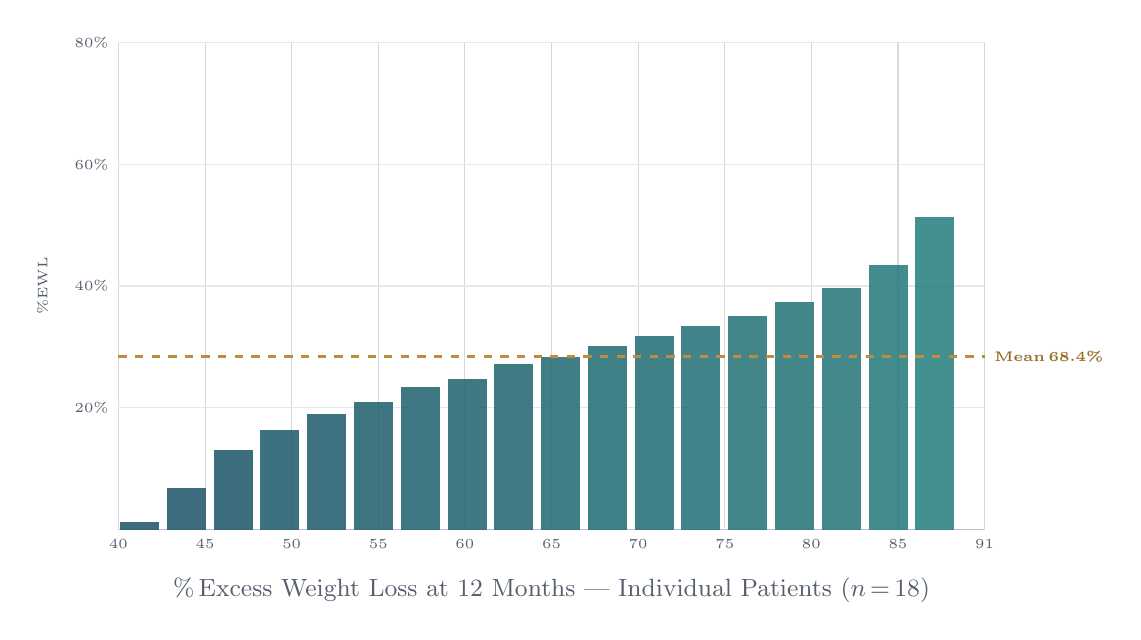
\begin{tikzpicture}[x=0.55cm, y=2.2pt]
  %% axes
  \draw[SurgBlue!30, line width=0.4pt] (0,0) -- (20,0);
  \foreach \x/\lbl in {0/40, 2/45, 4/50, 6/55, 8/60, 10/65, 12/70, 14/75,
                        16/80, 18/85, 20/91}{
    \draw[SurgBlue!20] (\x,0) -- (\x,80);
    \node[below, font=\tiny\color{GrayText}] at (\x,0) {\lbl};
  }
  %% grid y
  \foreach \y in {20,40,60,80}{
    \draw[SurgBlue!12] (0,\y) -- (20,\y);
    \node[left, font=\tiny\color{GrayText}] at (0,\y) {\y\%};
  }

  %% bars (18 patients, sorted %EWL values)
  \foreach \i/\ewl in {
    0/41.2, 1/46.8, 2/53.1, 3/56.4, 4/58.9, 5/61.0, 6/63.4,
    7/64.7, 8/67.2, 9/68.4, 10/70.1, 11/71.8, 12/73.5,
    13/75.0, 14/77.3, 15/79.6, 16/83.4, 17/91.3}{
    \pgfmathsetmacro{\bx}{\i * 1.08 + 0.04}
    \pgfmathsetmacro{\bxend}{\bx + 0.9}
    \pgfmathsetmacro{\bh}{\ewl - 40}
    \pgfmathsetmacro{\intensity}{40 + int(60*\i/17)}
    \fill[SurgTeal!\intensity!SurgBlue, opacity=0.88]
      (\bx, 0) rectangle (\bxend, \bh);
  }

  %% mean line
  \draw[SurgGold, line width=1.2pt, dashed] (0,{68.4-40}) -- (20,{68.4-40});
  \node[right, font=\tiny\bfseries\color{SurgGold!80!black}]
    at (20,{68.4-40}) {Mean\,68.4\%};

  %% axis label
  \node[below=14pt, font=\small\color{GrayText}] at (10,0)
    {\%\,Excess Weight Loss at 12 Months --- Individual Patients ($n$\,=\,18)};
  \node[above, font=\tiny\color{GrayText}, rotate=90] at (-1.4, 40) {\%EWL};
\end{tikzpicture}
\end{center}

\vspace{8pt}

%% ─────────────────────────────────────────────────────────────────────────────
%% SECTION 8 – DISCUSSION
%% ─────────────────────────────────────────────────────────────────────────────
\section{Discussion}

This single-centre retrospective case series demonstrates that laparoscopic sleeve
gastrectomy can be performed with low morbidity and excellent 12-month weight-loss
outcomes within a high-volume academic bariatric programme. Our mean \%EWL of
$68.4 \pm 12.7\%$ compares favourably with published meta-analytic estimates of
$60$--$70\%$ at one year.

The two major complications (11.1\%) are consistent with published series from
comparable centres, which report major complication rates of $5$--$15\%$ for LSG.
The single gastric leak was identified on day 3 and managed successfully by
re-laparoscopy, reflecting the importance of early recognition and a low threshold
for surgical re-exploration.

Comorbidity resolution rates were high: $66.7\%$ of patients with T2DM achieved full
remission, and $72.7\%$ of hypertensive patients either resolved or achieved significant
medication reduction at 12 months. These results align with the metabolic benefits
widely reported in the bariatric literature.

Limitations of this series include its retrospective design, single-surgeon experience,
small sample size, and 12-month maximum follow-up. A prospective randomised study
comparing LSG with Roux-en-Y gastric bypass within this institution is planned
(MAMC-SURG-2025-0012, pending ethics approval).

%% ─────────────────────────────────────────────────────────────────────────────
%% SECTION 9 – CONCLUSIONS
%% ─────────────────────────────────────────────────────────────────────────────
\section{Conclusions}

\begin{tcolorbox}[tealbox]
\begin{itemize}[leftmargin=16pt, itemsep=3pt, topsep=2pt]
  \item[\textcolor{SurgTeal}{\faCheckCircle}]
    LSG was performed safely in all 18 patients with zero intraoperative mortality
    and zero conversions to open surgery.
  \item[\textcolor{SurgTeal}{\faCheckCircle}]
    Mean \%EWL of $68.4\%$ at 12 months confirms the procedure's efficacy in
    a real-world academic setting.
  \item[\textcolor{SurgTeal}{\faCheckCircle}]
    Comorbidity resolution was substantial: T2DM remission $66.7\%$, hypertension
    resolution $72.7\%$, OSA resolution $71.4\%$.
  \item[\textcolor{SurgGold}{\faExclamationCircle}]
    Major complication rate of $11.1\%$ highlights the need for continued
    staple-line technique refinement and vigilant postoperative monitoring.
  \item[\textcolor{SurgBlue}{\faArrowCircleRight}]
    Prospective controlled study is warranted to compare LSG and RYGB in
    this patient population.
\end{itemize}
\end{tcolorbox}

\vspace{8pt}

%% ─────────────────────────────────────────────────────────────────────────────
%% SECTION 10 – AUTHOR CONTRIBUTIONS & DISCLOSURES
%% ─────────────────────────────────────────────────────────────────────────────
\section{Author Contributions \& Disclosures}

\begin{minipage}[t]{0.47\textwidth}
  \subsection*{Author Contributions}
  \small
  \textbf{A.~Voss:} Concept, surgical procedures, data analysis, manuscript preparation.\\
  \textbf{C.~Mendez:} Data collection, literature review, manuscript revision.\\
  \textbf{P.~Okafor:} Statistical analysis, figure preparation.\\
  \textbf{S.~Chen:} Dietetic assessment, postoperative follow-up, comorbidity data.\\
  \textbf{R.~Hargreaves:} Critical review, supervision.
\end{minipage}%
\hfill%
\begin{minipage}[t]{0.47\textwidth}
  \subsection*{Declarations}
  \small
  \textbf{Conflict of interest:} All authors declare no financial or personal
  conflict of interest related to the devices or techniques described.\\[4pt]
  \textbf{Funding:} No external or institutional funding was received for this study.\\[4pt]
  \textbf{Ethics approval:} Granted by the Meridian AMC Institutional Review Board
  (Ref: MAMC-SURG-2023-0041). All patients provided written informed consent.\\[4pt]
  \textbf{Data availability:} Anonymised case data available on reasonable
  request to the corresponding author.
\end{minipage}

\vspace{8pt}

%% ─────────────────────────────────────────────────────────────────────────────
%% REFERENCES
%% ─────────────────────────────────────────────────────────────────────────────
\section{References}

\begin{enumerate}[leftmargin=20pt, itemsep=2pt, label={\color{SurgBlue}\arabic*.}]
  \small
  \item Angrisani L, Santonicola A, Iovino P, et al.
    IFSO Worldwide Survey 2016: primary, endoluminal, and revisional procedures.
    \textit{Obes Surg.} 2018;28(12):3783--3794.
  \item Sarkhosh K, Birch DW, Shi X, Karmali S.
    The impact of sleeve gastrectomy on hypertension: a systematic review.
    \textit{Obes Surg.} 2012;22(5):832--837.
  \item Buchwald H, Avidor Y, Braunwald E, et al.
    Bariatric surgery: a systematic review and meta-analysis.
    \textit{JAMA.} 2004;292(14):1724--1737.
  \item Dindo D, Demartines N, Clavien PA.
    Classification of surgical complications: a new proposal with evaluation
    in a cohort of 6336 patients and results of a survey.
    \textit{Ann Surg.} 2004;240(2):205--213.
  \item Shi X, Karmali S, Sharma AM, Birch DW.
    A review of laparoscopic sleeve gastrectomy for morbid obesity.
    \textit{Obes Surg.} 2010;20(8):1171--1177.
  \item Rosenthal RJ; International Sleeve Gastrectomy Expert Panel, et al.
    International Sleeve Gastrectomy Expert Panel Consensus Statement:
    best practice guidelines based on experience of $>$12{,}000 cases.
    \textit{Surg Obes Relat Dis.} 2012;8(1):8--19.
  \item Schauer PR, Bhatt DL, Kirwan JP, et al.
    Bariatric surgery versus intensive medical therapy for diabetes ---
    5-year outcomes.
    \textit{N Engl J Med.} 2017;376(7):641--651.
\end{enumerate}

\vspace{10pt}

%% ─────────────────────────────────────────────────────────────────────────────
%% FOOTER STRIP
%% ─────────────────────────────────────────────────────────────────────────────
\begin{tikzpicture}[overlay, remember picture]
  \fill[SurgBlue]
    ([yshift=14pt]current page.south west)
    rectangle
    ([yshift=0pt]current page.south east);
  \node[anchor=south, text=white!70!SurgBlue,
        font=\scriptsize, yshift=2pt]
    at (current page.south) {%
      Meridian Academic Medical Centre\enspace\textbullet\enspace
      Surgical Case Series Report\enspace\textbullet\enspace
      MAMC-SURG-2023-0041\enspace\textbullet\enspace
      For Peer Review Only%
    };
\end{tikzpicture}

\end{document}
